\documentclass[12pt]{article}
\usepackage{amsmath}
\usepackage{graphicx}
\usepackage{hyperref}
\usepackage{listings}
\usepackage{color}
\usepackage{pythonhighlight}

\title{Operating System Course Report - First Half of the Semester}
\author{B class}
\date{\today}

\begin{document}

\maketitle
\newpage

\tableofcontents
\newpage

\section{Introduction}
This report summarizes the topics covered during the first half of the Operating System course. It includes theoretical concepts, practical implementations, and assignments. The course focuses on the fundamentals of operating systems, including system architecture, process management, CPU scheduling, and deadlock handling.

\section{Course Overview}
\subsection{Objectives}
The main objectives of this course are:
\begin{itemize}
    \item To understand the basic components and architecture of a computer system.
    \item To learn process management, scheduling, and inter-process communication.
    \item To explore file systems, input/output management, and virtualization.
    \item To study the prevention and handling of deadlocks in operating systems.
\end{itemize}

\subsection{Course Structure}
The course is divided into two halves. This report focuses on the first half, which covers:
\begin{itemize}
    \item Basic Concepts and Components of Computer Systems
    \item System Performance and Metrics
    \item System Architecture of Computer Systems
    \item Process Description and Control
    \item Scheduling Algorithms
    \item Process Creation and Termination
    \item Introduction to Threads
    \item File Systems
    \item Input and Output Management
    \item Deadlock Introduction and Prevention
    \item User Interface Management
    \item Virtualization in Operating Systems
\end{itemize}

\section{Topics Covered}

\subsection{Basic Concepts and Components of Computer Systems}
This section explains the fundamental components that make up a computer system, including the CPU, memory, storage, and input/output devices.

\subsection{System Performance and Metrics}
This section introduces various system performance metrics used to measure the efficiency of a computer system, including throughput, response time, and utilization.

\subsection{System Architecture of Computer Systems}
Describes the architecture of modern computer systems, focusing on the interaction between hardware and the operating system.

\subsection{Process Description and Control}
Processes are a central concept in operating systems. This section covers:
\begin{itemize}
    \item Process states and state transitions
    \item Process control block (PCB)
    \item Context switching
\end{itemize}

\subsection{Scheduling Algorithms}
	This section covers:
	\subsubsection{First-Come, First-Served (FCFS)}
	\subsubsection{Shortest Job Next (SJN)}
	\subsubsection{Round Robin (RR)}
        \begin{figure} [h]
        \centering
        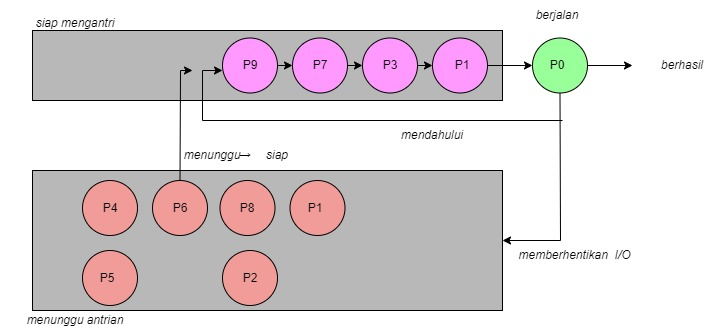
\includegraphics[width=0.75\textwidth]{assets/Round Robin diagram.jpg}
        \label{fig:diagram}
        \end{figure}
		Round robin scheduling adalah versi preemptive dari first-come, first-served scheduling. Proses-proses dijalankan dalam urutan first-in-first-out, tetapi setiap proses hanya diizinkan berjalan dalam jangka waktu yang terbatas. Interval waktu ini dikenal sebagai time-slice atau quantum. Jika suatu proses tidak selesai atau tidak diblokir karena operasi I/O dalam jangka waktu tersebut, maka time-slice akan habis, dan proses tersebut akan dipreempt. Proses yang dipreempt ini ditempatkan di bagian belakang antrian dan harus menunggu semua proses yang sudah ada di dalam antrian untuk berputar melalui CPU
		\par Jika suatu proses diblokir karena operasi I/O sebelum time-slice habis, maka tentu saja proses tersebut masuk ke dalam keadaan terblokir karena operasi I/O tersebut. Setelah operasi tersebut selesai, proses ini akan ditempatkan di akhir antrian dan menunggu gilirannya.
		\par Dalam round robin scheduling, kinerja interaktif tergantung pada panjang quantum dan jumlah proses dalam antrian. Quantum yang terlalu panjang membuat algoritma ini berperilaku seperti first come, first served scheduling, karena sangat mungkin bahwa suatu proses akan diblokir atau selesai sebelum time-slice habis. Quantum yang kecil memungkinkan sistem berputar melalui proses dengan cepat, yang bagus untuk proses interaktif. Sayangnya, ada overhead dalam context switching, dan melakukan hal ini terlalu sering meningkatkan persentase waktu sistem yang digunakan untuk context switching dibandingkan dengan pekerjaan nyata.
		
		\subsubsection*{Karakteristik Algoritma Penjadwalan CPU Round Robin}
		\begin{itemize}
			\item Sederhana, mudah diimplementasikan, dan bebas dari kekurangan sumber daya karena semua proses mendapat porsi CPU yang adil.
			\item Salah satu teknik yang paling umum digunakan dalam penjadwalan CPU adalah round robin.
			\item Hal ini bersifat preemptif karena proses hanya ditugaskan ke CPU untuk jangka waktu tertentu saja maksimal.
			\item Kerugiannya adalah lebih besarnya biaya overhead pelestarian konteks.
		\end{itemize}
		
		\subsubsection*{Keuntungan Algoritma Penjadwalan CPU Round Robin}
		\begin{itemize}
			\item Ada keadilan karena setiap proses mendapat bagian yang sama dari CPU.
			\item Proses yang baru dibuat ditambahkan ke akhir antrean siap.
			\item Penjadwalan round-robin umumnya menggunakan Pembagian waktu, yang memberikan setiap slot pekerjaan waktu atau quantum. 
			\item Saat melakukan penjadwalan round-robin, penempatan waktu tertentu dialokasikan untuk pekerjaan yang berbeda-beda. 
			\item Setiap proses mendapat kesempatan untuk menjadwalkan ulang setelah waktu tertentu tertentu dalam penjadwalan ini. 
		\end{itemize}
		
		\subsubsection*{Kekurangan Algoritma Penjadwalan CPU Round Robin}
		\begin{itemize}
			\item Ada waktu tunggu dan waktu respon yang lebih besar.
			\item Throughputnya rendah.
			\item Ada Peralihan Konteks.
			\item Bagan Gantt tampaknya terlalu besar (jika waktu penempatan lebih sedikit untuk penjadwalan. Misalnya: 1 ms untuk penjadwalan besar.)
			\item Penjadwalan yang memakan waktu untuk ukuran kecil.
		\end{itemize}

\subsection{Process Creation and Termination}
Details how processes are created and terminated by the operating system, including:
\begin{itemize}
    \item Process spawning
    \item Process termination conditions
\end{itemize}

\subsection{Introduction to Threads}
This section introduces the concept of threads and their relation to processes, covering:
\begin{itemize}
    \item Single-threaded vs. multi-threaded processes
    \item Benefits of multithreading
\end{itemize}

\begin{figure}[h]
    \centering
    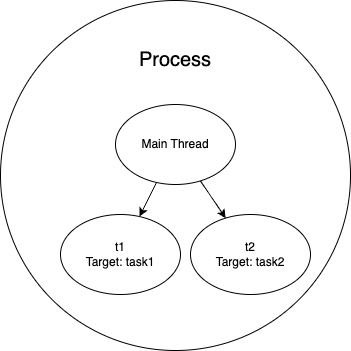
\includegraphics[width=0.5\textwidth]{/Users/khawaritzmi/Unhas/os_report_mid2024/b_class/asset/example.png}  % Sesuaikan nama file dan ukurannya
    \caption{Ini adalah gambar contoh dari multithreading.}
    \label{fig:contoh_gambar}
\end{figure}

Seperti yang terlihat pada Gambar \ref{fig:contoh_gambar}, inilah cara menambahkan gambar dengan keterangan.

\subsection{File Systems}
File systems provide a way for the operating system to store, retrieve, and manage data. This section explains:
\begin{itemize}
    \item File system structure
    \item File access methods
    \item Directory management
\end{itemize}

\subsection{Input and Output Management}
Input and output management is key for handling the interaction between the system and external devices. This section includes:
\begin{itemize}
    \item Device drivers
    \item I/O scheduling
\end{itemize}

\subsection{Deadlock Introduction and Prevention}
Explores the concept of deadlocks and methods for preventing them:
\begin{itemize}
    \item Deadlock conditions
    \item Deadlock prevention techniques
\end{itemize}

\subsection{User Interface Management}
This section discusses the role of the operating system in managing the user interface. Topics covered include:
\begin{itemize}
    \item Graphical User Interface (GUI)
    \item Command-Line Interface (CLI)
    \item Interaction between the user and the operating system
\end{itemize}

\subsection{Virtualization in Operating Systems}
Virtualization allows multiple operating systems to run concurrently on a single physical machine. This section explores:
\begin{itemize}
    \item Concept of virtualization
    \item Hypervisors and their types
    \item Benefits of virtualization in modern computing
\end{itemize}

\section{Assignments and Practical Work}
\subsection{Assignment 1: Process Scheduling}
Students were tasked with implementing various process scheduling algorithms (e.g., FCFS, SJN, and RR) and comparing their performance under different conditions.
\subsubsection{Group 5}
\subsubsection{Proses yang Diberikan}
Proses-proses yang perlu dijadwalkan ditampilkan pada Tabel \ref{tab:proses}.

\begin{table}[htbp]
    \centering
    \begin{tabular}{|c|c|c|}
        \hline
        PID & Waktu Kedatangan & Waktu Burst \\
        \hline
        1   & 0                & 5           \\
        2   & 2                & 3           \\
        3   & 4                & 1           \\
        \hline
    \end{tabular}
    \caption{Daftar proses yang akan dijadwalkan}
    \label{tab:proses}
\end{table}

\subsubsection{Soal}
\begin{itemize}
    \item Implementasikan algoritma penjadwalan proses berikut dalam Python:
        \begin{enumerate}
            \item First Come First Serve (FCFS)
            \item Shortest Job Next (SJN)
            \item Round Robin (RR) dengan kuantum waktu 2 unit
        \end{enumerate}
        
\textbf{Jawaban}
    \item Untuk setiap algoritma, hitung dan tampilkan hal berikut untuk setiap proses:
        \begin{itemize}
            \item Waktu Penyelesaian (Completion Time)
            \item Waktu Putar Balik (Turnaround Time)
            \item Waktu Tunggu (Waiting Time)
        \end{itemize}
    \item Bandingkan kinerja ketiga algoritma tersebut menggunakan set proses yang berbeda.
\end{itemize}

\textbf{Implementasi Python}

\subsubsection{FCFS}
Berikut adalah kode Python untuk algoritma First Come First Serve (FCFS).

\begin{python}[language=Python, caption=Kode Python untuk penjadwalan FCFS]
class Process:
    def __init__(self, pid, arrival_time, burst_time):
        self.pid = pid
        self.arrival_time = arrival_time
        self.burst_time = burst_time
        self.completion_time = 0
        self.turnaround_time = 0
        self.waiting_time = 0

def fcfs_scheduling(processes):
    current_time = 0
    for process in processes:
        if current_time < process.arrival_time:
            current_time = process.arrival_time
        process.completion_time = current_time + process.burst_time
        process.turnaround_time = process.completion_time - process.arrival_time
        process.waiting_time = process.turnaround_time - process.burst_time
        current_time += process.burst_time

def print_process_info(processes):
    print(f"{'PID':<10}{'Arrival':<10}{'Burst':<10}{'Completion':<15}{'Turnaround':<15}{'Waiting':<10}")
    for p in processes:
        print(f"{p.pid:<10}{p.arrival_time:<10}{p.burst_time:<10}{p.completion_time:<15}{p.turnaround_time:<15}{p.waiting_time:<10}")

# Contoh penggunaan
process_list = [
    Process(1, 0, 5),
    Process(2, 2, 3),
    Process(3, 4, 1),
]

fcfs_scheduling(process_list)
print_process_info(process_list)
\end{python}

\subsubsection{Shortest Job Next (SJN)}
Berikut adalah kode Python untuk algoritma Shortest Job Next (SJN).

\begin{python}[language=Python, caption=Kode Python untuk penjadwalan SJN]
def sjn_scheduling(processes):
    processes.sort(key=lambda x: (x.arrival_time, x.burst_time))
    current_time = 0
    while processes:
        available_processes = [p for p in processes if p.arrival_time <= current_time]
        if available_processes:
            next_process = min(available_processes, key=lambda x: x.burst_time)
            processes.remove(next_process)
            if current_time < next_process.arrival_time:
                current_time = next_process.arrival_time
            next_process.completion_time = current_time + next_process.burst_time
            next_process.turnaround_time = next_process.completion_time - next_process.arrival_time
            next_process.waiting_time = next_process.turnaround_time - next_process.burst_time
            current_time += next_process.burst_time
        else:
            current_time += 1

# Contoh penggunaan
process_list = [
    Process(1, 0, 5),
    Process(2, 2, 3),
    Process(3, 4, 1),
]

sjn_scheduling(process_list)
print_process_info(process_list)
\end{python}

\subsubsection{Round Robin (RR)}
Berikut adalah kode Python untuk algoritma Round Robin (RR) dengan kuantum waktu 2.

\begin{python}[language=Python, caption=Kode Python untuk penjadwalan Round Robin (RR)]
def rr_scheduling(processes, time_quantum):
    queue = processes[:]
    current_time = 0
    while queue:
        process = queue.pop(0)
        if process.burst_time > time_quantum:
            process.burst_time -= time_quantum
            current_time += time_quantum
            queue.append(process)
        else:
            current_time += process.burst_time
            process.completion_time = current_time
            process.turnaround_time = process.completion_time - process.arrival_time
            process.waiting_time = process.turnaround_time - process.burst_time

# Contoh penggunaan
process_list = [
    Process(1, 0, 5),
    Process(2, 2, 3),
    Process(3, 4, 1),
]

rr_scheduling(process_list, 2)
print_process_info(process_list)
\end{python}

\subsubsection{Hasil}
Tabel \ref{tab:hasil_perbandingan} menunjukkan hasil perbandingan antara algoritma FCFS, SJN, dan Round Robin untuk proses yang diberikan.

\begin{table}[htbp]
    \centering
    \begin{tabular}{|c|c|c|c|c|c|c|}
        \hline
        Algoritma & PID & A Time & B Time & C Time & T Time & W Time \\
        \hline
        FCFS      & 1   & 0            & 5          & 5               & 5               & 0            \\
                  & 2   & 2            & 3          & 8               & 6               & 3            \\
                  & 3   & 4            & 1          & 9               & 5               & 4            \\
        \hline
        SJN       & 1   & 0            & 5          & 9               & 9               & 4            \\
                  & 2   & 2            & 3          & 8               & 6               & 3            \\
                  & 3   & 4            & 1          & 5               & 1               & 0            \\
        \hline
        RR        & 1   & 0            & 5          & 9               & 9               & 4            \\
                  & 2   & 2            & 3          & 8               & 6               & 3            \\
                  & 3   & 4            & 1          & 5               & 1               & 0            \\
        \hline
    \end{tabular}
    \caption{Perbandingan Hasil Penjadwalan untuk FCFS, SJN, dan RR}
    \label{tab:hasil_perbandingan}
\end{table}

\subsection{Assignment 2: Deadlock Handling}
In this assignment, students were asked to simulate different deadlock scenarios and explore various prevention methods.

\subsubsection{Group 5}

\begin{enumerate}
    \item Pencegahan Deadlock menggunakan Algoritma Banker
    \item Pencegahan Deadlock melalui Pengecekan Sumber Daya
\end{enumerate}
Tugas Anda adalah mensimulasikan kedua metode di atas dan menunjukkan bagaimana deadlock dapat dihindari atau dicegah.


\textbf{Jawaban}
\subsubsection{Deadlock}
Deadlock terjadi ketika sekumpulan proses saling menunggu sumber daya yang dimiliki proses lain, dan tidak ada proses yang bisa melanjutkan eksekusinya. Kondisi-kondisi untuk terjadinya deadlock adalah:
\begin{itemize}
    \item Mutual Exclusion (Eksklusi Saling Terkait): Hanya satu proses pada satu waktu yang dapat menggunakan sumber daya.
    \item Hold and Wait (Menahan dan Menunggu): Proses yang menahan sumber daya juga dapat menunggu sumber daya lain.
    \item No Preemption (Tanpa Pemaksaan): Sumber daya tidak dapat diambil paksa dari proses yang memegangnya.
    \item Circular Wait (Tunggu Melingkar): Ada rantai proses di mana setiap proses menunggu sumber daya yang dipegang oleh proses lain dalam rantai.
\end{itemize}

\textbf{Metode Pencegahan Deadlock}

Berikut adalah dua metode pencegahan yang diterapkan pada skenario deadlock:

\subsubsection{Algoritma Banker's untuk Pencegahan Deadlock}
Algoritma Banker's mengevaluasi permintaan proses dan hanya mengabulkannya jika sistem dapat tetap berada dalam keadaan aman setelah mengalokasikan sumber daya tersebut.

\begin{python} caption=Implementasi Algoritma Banker]
class BankersAlgorithm:
    def __init__(self, processes, available, max_need, allocation):
        self.processes = processes
        self.available = available
        self.max_need = max_need
        self.allocation = allocation
        self.need = [[self.max_need[i][j] - self.allocation[i][j] for j in range(len(self.max_need[0]))] for i in range(len(self.processes))]

    def is_safe(self):
        work = self.available[:]
        finish = [False] * len(self.processes)
        safe_sequence = []

        while len(safe_sequence) < len(self.processes):
            safe = False
            for i in range(len(self.processes)):
                if not finish[i] and all(self.need[i][j] <= work[j] for j in range(len(work))):
                    for j in range(len(work)):
                        work[j] += self.allocation[i][j]
                    finish[i] = True
                    safe_sequence.append(self.processes[i])
                    safe = True
            if not safe:
                return False, []
        return True, safe_sequence

# Contoh penggunaan
processes = ['P0', 'P1', 'P2', 'P3']
available = [3, 3, 2]
max_need = [
    [7, 5, 3],
    [3, 2, 2],
    [9, 0, 2],
    [2, 2, 2]
]
allocation = [
    [0, 1, 0],
    [2, 0, 0],
    [3, 0, 2],
    [2, 1, 1]
]

bankers = BankersAlgorithm(processes, available, max_need, allocation)
is_safe, safe_sequence = bankers.is_safe()
if is_safe:
    print("Sistem aman. Urutan aman:", safe_sequence)
else:
    print("Sistem tidak aman. Deadlock mungkin terjadi.")
\end{python}

\subsubsection {Pencegahan Deadlock melalui Pengecekan Sumber Daya (Resource Allocation Check)}
Metode ini mengecek apakah alokasi sumber daya saat ini dapat mengakibatkan deadlock dengan memeriksa apakah semua proses dapat menyelesaikan eksekusi mereka.

\begin{python}[language=Python, caption=Implementasi Pengecekan Alokasi Sumber Daya]
def resource_allocation_check(processes, available, max_need, allocation):
    need = [[max_need[i][j] - allocation[i][j] for j in range(len(available))] for i in range(len(processes))]
    finish = [False] * len(processes)
    work = available[:]
    
    while True:
        progress = False
        for i in range(len(processes)):
            if not finish[i] and all(need[i][j] <= work[j] for j in range(len(available))):
                for j in range(len(available)):
                    work[j] += allocation[i][j]
                finish[i] = True
                progress = True
        if not progress:
            break

    return all(finish)

# Contoh penggunaan
processes = ['P0', 'P1', 'P2', 'P3']
available = [3, 3, 2]
max_need = [
    [7, 5, 3],
    [3, 2, 2],
    [9, 0, 2],
    [2, 2, 2]
]
allocation = [
    [0, 1, 0],
    [2, 0, 0],
    [3, 0, 2],
    [2, 1, 1]
]

if resource_allocation_check(processes, available, max_need, allocation):
    print("Sistem aman. Semua proses dapat diselesaikan.")
else:
    print("Deadlock mungkin terjadi.")
\end{python}

\subsubsection{Hasil Simulasi}
Hasil simulasi dari algoritma Banker's dan pengecekan sumber daya menunjukkan bahwa sistem dapat berada dalam keadaan aman jika alokasi sumber daya dilakukan dengan hati-hati. Jika ada deadlock yang mungkin terjadi, sistem akan mencegah permintaan lebih lanjut atau melakukan pre-emption sumber daya.

\subsection{Assignment 3: Multithreading and Amdahl's Law}
This assignment involved designing a multithreading scenario to solve a computationally intensive problem. Students then applied **Amdahl's Law** to calculate the theoretical speedup of the program as the number of threads increased.

\subsection{Assignment 4: Simple Command-Line Interface (CLI) for User Interface Management}
Students were tasked with creating a simple **CLI** for user interface management. The CLI should support basic commands such as file manipulation (creating, listing, and deleting files), process management, and system status reporting.

\subsection{Assignment 5: File System Access}
In this assignment, students implemented file system access routines, including:
\begin{itemize}
    \item File creation and deletion
    \item Reading from and writing to files
    \item Navigating directories and managing file permissions
\end{itemize}

\section{Conclusion}
The first half of the course introduced core operating system concepts, including process management, scheduling, multithreading, and file system access. These topics provided a foundation for more advanced topics to be covered in the second half of the course.

\begin{thebibliography}{9}
    \bibitem{ref1} GeeksforGeeks. (n.d.-a). First Come First Serve | CPU scheduling (non-preemptive). Retrieved October 1, 2024, from https://www.geeksforgeeks.org/first-come-first-serve-cpu-scheduling-non-preemptive/
    \bibitem{ref2} GeeksforGeeks. (n.d.-b). Program for FCFS CPU scheduling | Set 1. Retrieved October 1, 2024, from https://www.geeksforgeeks.org/program-for-fcfs-cpu-scheduling-set-1/
    \bibitem{ref3} GeeksforGeeks. (n.d.-c). Shortest Job Next (SJN) in Operating System. Retrieved October 1, 2024, from https://www.geeksforgeeks.org/shortest-job-next-sjn-in-operating-system/
    \bibitem{ref4} GeeksforGeeks. (n.d.-d). Program for Shortest Job First (SJF) CPU scheduling | Set 1 (non-preemptive). Retrieved October 1, 2024, from https://www.geeksforgeeks.org/program-for-shortest-job-first-or-sjf-cpu-scheduling-set-1-non-preemptive/
    \bibitem{ref5} GeeksforGeeks. (n.d.-e). Program for Round Robin scheduling for the same arrival time. Retrieved October 1, 2024, from https://www.geeksforgeeks.org/program-for-round-robin-scheduling-for-the-same-arrival-time/
    \bibitem{ref6} GeeksforGeeks. (n.d.-f). Round Robin scheduling with different arrival times. Retrieved October 1, 2024, from https://www.geeksforgeeks.org/round-robin-scheduling-with-different-arrival-times/ 
    \bibitem{ref7}Marty, J. (n.d.). Process scheduling. Clemson University. Retrieved October 1, 2024, from https://people.computing.clemson.edu/~jmarty/courses/commonCourse
    Content/AdvancedModule-LinuxSysAdmin/NotesProcessScheduling.pdf 
    \bibitem{ref8} Silberschatz, A., Galvin, P. B., and Gagne, G. (2018). Operating System Concepts (10th ed.). Wiley.
\end{document}